%\RequirePackage[l2tabu, orthodox]{nag}
\documentclass[a4paper,12pt]{scrreprt}
\usepackage[utf8]{inputenc}   % input encoding
\usepackage[T1]{fontenc}      % font encoding
\usepackage[english]{babel}		% English language 
\usepackage{lmodern}					% font looks better on screen
\usepackage{microtype}				% improve kerning
\usepackage[left=3.5cm,right=2.5cm]{geometry} % setup page geometry
\usepackage{nomencl}          % nomenclature
% if using natbib
\usepackage{natbib}           % bibliography for scientists
% if using biblatex
%\usepackage[backend=bibtex,style=authoryear,bibstyle=nature,natbib=true]{biblatex}
%\usepackage{csquotes}         % dunno what this does
%--------------------------------------------------
% more features
\usepackage{amsmath}					% all the fancy math stuff
\usepackage{caption}          % customize captions
\usepackage{color}						% enable color
%\usepackage{enumerate}				% customize numbered lists
\usepackage{graphicx}					% fancy graphics
\usepackage{listings}         % code listings
\usepackage{tabularx}         % extended tables
%\usepackage{tikz}             % draw stuff with tikz
\usepackage{url}							% URL handling
\usepackage{xspace}						% to space or not to space
\usepackage{hyperref} 				% should be loaded last
%--------------------------------------------------

%
% new colors and commands, mostly formatting
%
\definecolor{lightgrey}{rgb}{0.9,0.9,0.9}
\renewcommand{\nomname}{List of Abbreviations}
\newcommand{\file}[1]{{\lstinline{#1}}}
\newcommand{\code}[1]{{\texttt{#1}}}
\newcommand{\tool}[1]{\textit{#1}}
\newcommand{\hamstr}{HaMStR\xspace}
\newcommand{\pname}{Orthograph\xspace}
\newcommand{\pfullname}{\emph{Ortho}logy prediction using a \emph{gr}aph-based \emph{a}pproach with \emph{p}rofile \emph{h}idden Markov models\xspace}
\newcommand{\myself}{Malte Petersen}
\newcommand{\mytitle}{Fast and efficient mapping of transcript sequences to ortholog groups}
\newcommand{\species}[1]{\textit{#1}}
\newcommand{\ie}[1]{\textit{i.e.,}}
\newcommand{\eg}[1]{\textit{e.g.,}}
\newcommand{\todo}[1]{\textbf{\color{red}[#1]}}

\makenomenclature
%
% setup biblatex
%
%--------------------------------------------------
% \bibliography{bib/diploma}
% \ExecuteBibliographyOptions{
% 	firstinits=true,
% 	backref=true,
% 	isbn=false,
% 	url=false,
% 	maxcitenames=2,
% 	maxbibnames=999,
% }
% \renewcommand{\bibfont}{\normalfont\footnotesize}
%-------------------------------------------------- 

%
% setup natbib citation format
%
\bibpunct{(}{)}{,}{a}{,}{,}

%
% setup caption format
%
\captionsetup{format=plain, font=small, labelfont=bf}

%
% setup code listings
%
\lstset{%
	language=perl,
	basicstyle=,                       % size of the fonts that are used for the code
	numbers=left,                      % where to put the line numbers
	numberstyle=\tiny,                 % size of the fonts that are used for the line numbers
	%stepnumber=2,                      % step between two line numbers. 
	numbersep=5pt,                     % how far the line numbers are from the code
	backgroundcolor=\color{lightgrey}, % choose the background color. Requires \usepackage{color}
	showspaces=false,                  % show spaces adding particular underscores
	showstringspaces=false,            % underline spaces within strings
	showtabs=false,                    % show tabs 
	frame=none,                        % none|leftline|topline|bottomline|lines|single, shadowbox 
	%frameround=tttt,                   % rounded corners; t=round, f=corner
	tabsize=2,                         % sets default tabsize to 2 spaces
	captionpos=t,                      % caption position (t|b)
	breaklines=true,                   % automatic line breaking
	breakatwhitespace=false,           % automatic breaks should not happen at whitespace
	%escapeinside={\%}{)}               % if you want to add a comment within your code
}

%
% setup hyperlinks, bookmarks and pdf metadata
%
\hypersetup{%
	bookmarks=true,
	pdfborder={0 0 0},
	pdftitle={\mytitle},
	pdfauthor={\myself},
	pdfcreator={pdflatex},
	pdfsubject={orthology prediction},
	pdfkeywords={orthology} {prediction} {est} {transcriptome} {hmm} {phylogenetics} {thesis} {1kite}
}
% alleviate compression so pdftk won't complain
\pdfobjcompresslevel=1

%
% doublespace
%
\linespread{1.3}

%--------------------------------------------------
% start of actual document
%-------------------------------------------------- 
\begin{document}

%
% title page
%
\begin{titlepage}
	\begin{center}
\null\vspace{2.23cm}
\textsf{\Huge\textbf{Fast and efficient mapping of transcript sequences to
ortholog groups}}\\
\vspace{8em}
\large{Malte Petersen}\\
\vfill
\normalsize{Diplomarbeit}\\
~\newline
\small
Rheinische Friedrich-Wilhelms-Universität Bonn\\
Mathematisch-Naturwissenschaftliche Fakultät\\
~\newline
angefertigt am\\
Zentrum für Molekulare Biodiversitätsforschung\\
Zoologisches Forschungsmuseum Alexander Koenig
\end{center}

\end{titlepage}

%
% paper notes, remove this later
%
%--------------------------------------------------
% \chapter*{Paper notes}
% 	Obstacles:
\begin{itemize}
	\item remote database performance
	\item local database performance: binify
	\item unique ids
	\item avoid redundancy
	\item soft threshold
\end{itemize}

Strategies for orthology prediction:

Tree reconciliation

\begin{itemize}
	\item topology of a gene tree compared with that of the chosen species tree
	\item reconciled by maximum parsimony $\rightarrow$ reflects ortholog
		relationships
	\item genome-wide application precluded by:
	\begin{itemize}
		\item horizontal gene transfer, especially in prokaryotes (widespread HGT
			invalidates the very notion of a species tree)
		\item computationally expensive
	\end{itemize}
\end{itemize}

\begin{description}
	\item[\cite{mirkin1995}] Tree-based approach to orthology prediction
	\item[\cite{page1998}] Tree reconciliation method
	\item[\cite{yuan1998}] Tree-based approach to orthology prediction
	\item[\cite{kuzniar2008}] Review of approaches
\end{description}

most studies employ simplifications/shortcuts $\rightarrow$ graph-based approaches:

Triangulation

\begin{itemize}
	\item OrthoDB 
	\item COG (KOG, EGO, etc)
\end{itemize}

Reciprocal best hit (RBH) 

\begin{itemize}
	\item RBH strategies recover only one-to-one orthologs (the bidirectional best
		hit)
	\item InParanoid (BLAST based)
\end{itemize}

Markov clustering:

\begin{itemize}
	\item OrthoMCL
\end{itemize}

Homoplasy: similarity in unrelated organisms. Homoplasies demonstrate adaptation
in the living world.

Homoplasy \citep{lankester1870}: It may be said that the term ``analogy'',
already in use, is sufficient to indicate what is here termed ``homoplasy''; but
analogy has had a wider signification given to it, in which it is found very
useful to employ it, and if could not be used with any accuracy in place of
homoplasy.  \emph{Any} two organs having the same function are analogous,
whether closely resembling each other in their structure and relation to other
parts or not, and it is well to retain the word in that wide sense. Homoplasy
includes all cases of close resemblance of form which are not traceable to
homogeny, all \emph{details} of agreement not homogenous, in structures which
are broadly homogenous, as well as in structures having no genetic affinity.

%-------------------------------------------------- 

%
% declaration of authorship
%
\chapter*{Declaration of authorship}
	\thispagestyle{empty}
%--------------------------------------------------
% Ich versichere hiermit an Eides statt, dass die vorliegende Diplomarbeit
% selbstständig verfasst und keine weiteren als die angegebenen Hilfsmittel
% benutzt sowie die Stellen der Arbeit, die in anderen Werken dem Wortlaut oder
% dem Sinn nach entnommen sind, durch Angaben der Quellen sichtbar gemacht
% wurden.
%-------------------------------------------------- 

I herewith declare that I have written this thesis independently and myself. I
did not use any other sources than those listed. All places where the exact
words or analogous text were taken from sources are indicated. I assure that
this thesis has not been submitted for examination elsewhere.

\vspace{4em}

\parbox[t]{0.3\textwidth}{\dotfill}

Bonn, \today

\myself

\vfill

\noindent
\textbf{1. Referee:} Prof. Dr. Bernhard Misof\\
Zentrum für Molekulare Biodiversitätsforschung\\
Zoologisches Forschungsmuseum Alexander Koenig\\

\noindent
\textbf{2. Referee:} PD Dr. Lars Podsiadlowski\\
Institut für Evolutionsbiologie und Zoo-Ökologie

	\clearpage

%
% license
%
\thispagestyle{empty}
\null
\vfill
\noindent
\href{http://creativecommons.org/licenses/by-sa/3.0/}{
\includegraphics[width=0.15\textwidth]{img/license-cc-attribution-sharealike.pdf}}\\
This work is licensed under a
\textbf{\href{http://creativecommons.org/licenses/by-sa/3.0/}{Creative Commons
Attribution-ShareAlike 3.0 Unported License}}. The full \LaTeX~source code
including figures and bibliography is hosted on GitHub at
\url{https://github.com/mptrsen/thesis}.


%
% dedication
%
%\thispagestyle{empty}
\null
\vfill
\begin{center}
for the unborn
\end{center}
\vfill


%
% start numbering pages in roman
%
\pagenumbering{roman}
\pagestyle{headings}

%
% table of contents
%
\phantomsection
\addcontentsline{toc}{chapter}{Contents}
\tableofcontents
\clearpage

%
% list of figures
%
\phantomsection
\addcontentsline{toc}{chapter}{List of figures}
\listoffigures
\clearpage

%
% list of tables
%
\phantomsection
\addcontentsline{toc}{chapter}{List of tables}
\listoftables
\clearpage

%
% list of abbrevs
%
\phantomsection
\addcontentsline{toc}{chapter}{List of abbreviations}
\markboth{\nomname}{\nomname}
\setlength{\nomitemsep}{-\parsep}
\nomenclature{1KITE}{1,000 insect transcriptome evolution}
\nomenclature{ACID}{Atomicity, Consistency, Isolation, Durability}
\nomenclature{BBH}{Bidirectional best hits}
\nomenclature{BLAST}{Basic local alignment search tool}
\nomenclature{B}{Byte}
\nomenclature{CPAN}{Comprehensive Perl Archive Network}
\nomenclature{CPU}{Central processing unit}
\nomenclature{DBD}{Database driver}
\nomenclature{DBI}{Database interface}
\nomenclature{DBMS}{Database management system}
\nomenclature{DNA}{Deoxyribonucleic acid}
\nomenclature{EST}{Expressed sequence tag}
\nomenclature{GB}{Gigabyte}
\nomenclature{GCC}{Gnu C compiler}
\nomenclature{GHz}{Gigahertz}
\nomenclature{GPL}{GNU General Public License}
\nomenclature{HPC}{High performance computing}
\nomenclature{HP}{Hewlett-Packard}
\nomenclature{ID}{Identifier}
\nomenclature{NCBI}{National Center for Biotechnology Information}
\nomenclature{OGS}{Official gene set}
\nomenclature{RAM}{Random access memory}
\nomenclature{RBH}{Reciprocal best hit}
\nomenclature{RDBMS}{Relational database management system}
\nomenclature{RNA}{Ribonucleic acid}
\nomenclature{SHA-256}{Secure hash algorithm} 
\nomenclature{SQL}{Structured query language} 
\nomenclature{Vim}{Vi improved}
\nomenclature{X}{Ambiguity character in amino acid sequences; may be any amino acid}
\nomenclature{ZFMK}{Zoologisches Forschungsmuseum A. Koenig}
\nomenclature{bp}{Basepair(s)}
\nomenclature{mRNA}{Messenger ribonucleic acid}

\printnomenclature[2cm]
\clearpage

%
% quote 8-)
%
\phantomsection
\thispagestyle{empty}
\null
\vfill
\begin{quote}
	\emph{Mutation:} it is the key to our evolution. It has enabled us to evolve
	from a single-celled organism into the dominant species on the planet. This
	process is slow, and normally taking thousands and thousands of years. But
	every few hundred millennia, evolution leaps forward.\\
	\null\hfill--- \citet{singer2000}
\end{quote}


%
% restart numbering in arabic
%
\pagenumbering{arabic}

%
% content
%
\chapter{Introduction}
	Since the advent of DNA sequencing technology and the reconstruction of
genealogical relationships based on nucleic or amino acid sequences, the
challenge has arisen to select appropriate, comparable molecular characters for
phylogenetic analyses. So-called orthologs are the only type of molecular
characters that can be used as evidence of a speciation event. 

A number of techniques has been developed to assess orthology in genomes. In
recent research, transcriptomes---which are only the subset of a genome that is
expressed at the time of RNA preservation---are frequently used because of lower
sequencing cost. However, methods that work in whole genomes cannot be applied
to transcriptomes because of the inherent incompleteness of transcriptomic data.
In the present thesis, I outline the concept of gene orthology and infer a
software pipeline that allows orthology prediction in transcriptome data.


	\section{Orthology}
		When reconstructing the evolution of species lineages, so called homologous
characters are used to reconstruct phylogenetic trees. The term homolog was
introduced by \citet{owen1848} and was used to describe ``the same organ in
different animals under different every variety of form and function''.
Similarly, analogs were defined as ``part or organ in one animal which has the
same function as another part or organ in a different animal''. At that time,
Owen had no notion of the concept of evolution, and in the famous \emph{Origin
of Species} \citep{darwin1859}, the term homology is never used. However, in a
review, \citet{owen1860} refers to homology as evidence of evolution.

A morphological character is the phenotypic reflection of genetic information.
Since the analysis of molecular data entered the field of phylogenetics during
the 1960s, these are used in numerous studies on species relationships.
Molecular characters, such as the DNA sequences of genes, are homologous if they
share a common origin. However, this is not sufficient to infer reliable
phylogenies based on molecular sequence data. Genes do not only dplicate during
a speciation event, but can be subject to a number of events in the course of
their evolutionary history, such as speciation, gene duplication, gene loss,
horizontal gene transfer as well as fusion, fission and other rearrangements of
genes \citep{koonin2005}.  These different types of relatedness between
sequences of molecular characters have made new definitions necessary (see
\autoref{fig:orthology}).

\begin{figure}[h]
	\centering
	\def\svgwidth{0.8\textwidth}
	\input{img/orthology-paralogy.pdf_tex}
	\caption[Orthology, paralogy, and xenology]{Subtypes of homology. The red
		arrow denotes horizontal gene transfer; AB1 is \emph{xenologous} to all
		other genes. B1 and C1 are \emph{orthologs}. Both C2 and C3 are
		\emph{inparalogs} to each other but \emph{co-orthologs} to B2, as are B1 and
		C1 compared to A1. B1 and B2 are outparalogs. Graphic adapted from
		\citet{fitch2000}.
	}
	\label{fig:orthology}
\end{figure}


Homologous genes in two or more species that are related by a speciation event
are called \emph{orthologs}\footnote{\emph{ortholog} n., \emph{orthologous}
adj.; the other terms are flexed accordingly.} \citep{fitch1970}. They reflect
species phylogeny directly and are most commonly used to infer phylogenetic
relationships between species. \emph{Paralogs} are also homologous genes, but
they are related by a gene duplication event within a species and are not
involved in horizontal radiation \citep{ohno1970}. Further distinction must be
made among paralogous genes \citep{remm2001}: paralogous genes that are related
by a lineage-specific duplication are called \emph{outparalogs} if the
duplication occurred prior to a given speciation event. On the contrary, genes
that result from a lineage-specific duplication subsequent to a given speciation
event are called \emph{inparalogs}. Additionally, two genes in a single species
that are paralogous to each other can be \emph{co-orthologs} to a gene in
another species. These distinctions are important when looking at internal
branches of a phylogenetic tree. 

A fourth subtype of homology is called \emph{xenology}. It is defined as the
condition in which the history of the genes involves horizontal, or
interspecies, gene transfer \citep{gray1983}. This is the only form of homology
in which the gene lineage cannot be traced back to a parent, but instead from
one organism to another.

In molecular phylogenetics, orthologous molecular sequences are used to
reconstruct genealogical relationships, because these sequences are the only
homologous sequences whose phylogeny reflects the genealogical relationships of
the species from which the sequences were obtained. Orthologs are also used to
study mechanisms of gene and genome evolution \citep{dessimoz2012}. Orthologs
tend to be more functionally similar than paralogs \citep{altenhoff2012}. This
is the so-called \emph{ortholog conjecture} \citep{tatusov1997}, and the reason
why the analysis of protein families often relies on orthology among the
investigated genes. In addition, housekeeping genes, i.e., genes that are
essential to keeping an organism alive, underlie stronger sequence conservation
due to selection pressure \citep{she2009} and are more likely to be orthologous
across species \citep{waterhouse2011}. 

	\section{How can orthology be assessed?}
		With next-generation, high-throughput technologies providing vast amounts of
sequence data, 

To make use of the information contained in the ortholog property, it is
important to classify conserved genes according to their homologous
relationships. It is worth mentioning here that homology is a concept of
quality, not quantity (\cite{reeck1987}) and thus indivisible. Two sequences can
be \emph{similar} by a percentage (e.g., amino acid positional identity), but
they are either homologous or they are not. The same follows for orthologs,
paralogs, and xenologs. This distinction is important because homology implies a
genealogical relationship, whereas similarity does not. Similarity can also be
the result of other evolutionary processes, such as convergence, which results
in \emph{analogy}. All variants of similarity can be grouped under the term
\emph{homoplasy}, which encompasses similarity (\emph{homos} (``equal''),
\emph{plasis} (``shaping'')) excluding homology and its subforms. In the present
thesis, the definition of homoplasy is used as it appears in \cite{page1998}.

A simple alignment or scoring (i.e., similarity) alone cannot separate
homologous from merely similar sequences (\cite{eisen1998}). To distinguish
homology from homoplasy, further logic is necessary: 

See figure \ref{fig:hamstr}.

	\section{Transcriptomes and additional challenges}
		Going a step back and asking why genomes are studied, many times the answer is
that one wants to understand the function of genes and proteins. The genome is
made up of long strands of deoxyribonucleic acid (DNA). It contains the
necessary instructions to create and maintain cells.  Proteins are produced
according to information on the DNA in a two-step process: during
\emph{transcription}, messenger ribonucleic acid (mRNA) is synthetisized. In the second step, \emph{translation}, the
mRNA is used by specialized organelles, namely ribosomes, to synthetisize
proteins from amino acids. In eukaryotes, this process includes \emph{splicing},
during which non-coding regions, so-called \emph{introns} are removed from the
mRNA. In bacteria and archaea, the mRNA requires typically no further processing
before translation. The resulting molecule contains only \emph{exons}, coding
regions of the genome that are relevant for translation. The ratio of exons to
introns varies across organisms; \eg, the human genome consists of only 1.1\% to
1.4\% exons and 24.4\% to 37.8\% introns, the rest is intergenic DNA
\citep{venter2001}. That means that in eukaryotes, the majority of the genome
does not code for proteins, and the functional analysis of the genes in an
eukaryote genome requires screening the nucleotide sequence data for those
non-coding regions.

The study of \emph{transcriptomes} circumvents these problems. A transcriptome
is the collection of all transcripts in a tissue sample at the time of RNA
preservation.  Transcriptomes are frequently used in phylogenetics and
phylogenomics to reconstruct species trees based on hundreds of
genes\footnote{The 1KITE project (1K Insect Transcriptome Evolution,
\url{http://1kite.org}) aims to sequence the transcriptomes of 1,000 insect
species and infer a robust backbone tree of insects. Preliminary analyses were
performed on a supermatrix of 1,478 genes.}.  The combination of low-cost
next-generation sequencing and the intron-free nature of transcriptomes allow
access to a high proportion of protein coding genes per sequenced mega-base pair
at a fraction of the cost for sequencing the corresponding genome.

Next-generation transcriptome sequencing technologies achieve their high
throughput by massively parallelizing the sequencing process. They cannot
sequence whole genomes in a single run, but produce a large number of so-called
\emph{reads}, short nucleotide sequences (20 to 1,000 bp in length, depending on
the technology used).  These fragments must be \emph{assembled} to form
so-called \emph{contigs}, contiguous sequences of nucleotides that most closely
resembles the nucleotide sequence present in the sequenced specimen. The
assembly process is a computationally complex problem that has not yet been
solved to perfection.  Reviews of different strategies have been written by,
\eg, \citet{zhang2011}.  The assembled data may be redundant due to, \eg,
alternative splicing products \citep{black2003} or multiple, non-overlapping
sequencing of C-terminus and N-terminus (the two ends of a DNA strand or gene).
Most assembly software cannot detect these issues reliably \citep{haiminen2011}. 

In addition to the processes explained above, next-generation transcriptome
sequencing and assembly output sequence data are not only fragmented and
possibly redundant (overlapping), but most importantly they are
\emph{incomplete} because not all genes may have been expressed at the time of
preservation. Due to this inherent incompleteness of transcriptomes, orthology
prediction approaches that are used on fully sequenced and annotated genomes
cannot be used.

\begin{figure}[t]
	\centering
	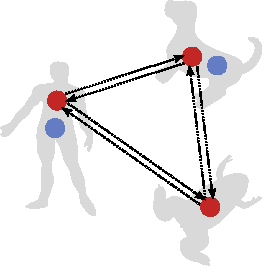
\includegraphics[width=0.4\textwidth]{img/triangulation-bbh.pdf}
	\caption[Bidirectional best hit (BBH) triangulation]{
		Bidirectional best hit (BBH) triangulation. To identify genes as orthologous
		in the presence of potential gene loss or incomplete data, they must be BBH
		in three species.  In this example, the red gene fulfills this criterion.
		The blue gene cannot be unambiguously identified as orthologous, as it is
		not present in the frog and paralogy is possible (compare to
		\autoref{fig:graph-based-strat}).  Graphic modified from
		\citet{altenhoff2012}.
	}
	\label{fig:triangulation-bbh}
\end{figure}


When performing a bidirectional search on a fully sequenced and annotated
complete genome as described above, it can happen that two genes that are
identified as BBH are paralogs because the corresponding orthologs have been
lost in both investigated species. This situation is called \emph{differential
gene loss}\cite{altenhoff2012} and best solved using a tree-based approach. In
the face of the aforementioned difficulties of a tree-based strategy, some
graph-based algorithms implement \emph{triangulation}
(\autoref{fig:triangulation-bbh}): to identify two genes as orthologous, they
must be BBH not only in two, but in three species. The third gene functions as
possible ``witness of non-orthology'' \citep{dessimoz2006}. A triangulation
strategy can also be applied to orthology prediction in transcriptomic data, the
incompleteness of which may be seen as a similar situation as potential gene
loss in fully sequenced and annotated genomes. This approach has been
implemented in \hamstr \citep{ebersberger2009}, which I will describe in the
following section.

	\section{\hamstr}
		HaMStR \citep{ebersberger2009} implements a graph-based approach using hidden
Markov models (HMMs, see section \ref{sec:hmms}). It is aimed specifically at
searching for orthologs in expressed sequence tag (EST) data, which is sequenced
using complementary DNA (cDNA) libraries. This cDNA is generated from mRNA and
therefore contains no introns. EST data can be redundant and fragmented, which
is why methods for orthology prediction in genomic data cannot be applied.

The HaMStR algorithm goes as follows:

\begin{enumerate}
	\item For each HMM, do the following:
		\begin{enumerate}
			\item Search the EST library. If matches were found, do the following for
				each:
			\begin{enumerate}
				\item Search the hit sequence against a BLAST database of all reference
					proteomes (the ``reciprocal BLAST''). 
				\item If matches were found: 

			\end{enumerate}
		\end{enumerate}
\end{enumerate}

\begin{figure}[h]
	\centering
	\def\svgwidth{0.8\textwidth}
	\input{img/triangulation.pdf_tex}
	\caption[Triangulation]{Triangulation:
		\begin{inparaenum}
			\item The transcript sequence space is searched using a hidden Markov
				model (HMM), which is a statistical representation of the reference
				sequences that were used to build it.
			\item A reference proteome is searched using the match sequence from the
				HMM search (reciprocal search).
			\item If the reciprocal search match sequence is one that was used to
				build the HMM, then orthology is assumed.
		\end{inparaenum}
	}
	\label{fig:hamstr}
\end{figure}

% enable this if you need it, it makes compilation a bit slower
%\usetikzlibrary{shapes,arrows}
\tikzstyle{rect} = [
	rectangle,
	draw,
	fill = green!15,
	text width = 9 em,
	text centered,
	minimum height = 3 em,
]
\tikzstyle{block} = [
	rectangle,
	draw,
	fill = blue!20,
	text width = 13em,
	text centered,
	rounded corners,
	minimum height = 3em,
]
\tikzstyle{decision} = [
	diamond,
	draw, 
	fill = blue!20, 
	text width = 4.5em,
	text centered,
	node distance = 14em,
	inner sep = 0pt
]
\tikzstyle{line} = [draw, -latex]
\tikzstyle{cloud} = [
	draw,
	ellipse,
	fill = red!20,
	text width = 7.5em,
	text badly centered,
	node distance = 3cm,
	minimum height = 2em
]

\hyphenation{ref-e-ren-ce tran-scrip-to-me or-tho-lo-gous}
\begin{tikzpicture}[node distance = 2cm, auto]
	% nodes
	\node[rect] (transcriptome) {Transcriptome library};
	\node[block, below of = transcriptome] (hmmsearch) {Search transcriptome library using next HMM};
	\node[rect, left of = hmmsearch, node distance = 14em] (orthologs) {pHMMs of orthologous sequences};
	\node[block, above of = orthologs] (orthodb) {Orthologous sequences of reference taxa from OrthoDB};
	\node[block, below of = hmmsearch, node distance = 4em] (hmmhits) {BLAST result(s) against next reference taxon};
	\node[decision, below of = hmmhits, node distance = 7em] (blast) {BLAST hit in HMM?};
	\node[rect, right of = hmmhits, node distance = 14em] (proteomes) {Proteomes of the reference taxa};
	\node[cloud, below of = blast, node distance=7em] (orthologous) {Orthologous, save \& process};
	\node[decision, below of = orthologous, node distance = 6em] (hmmsleft) {HMMs left?};
	\node[decision, left of = blast, node distance = 16em] (reftaxaleft) {Reference taxa left?};
	\node[cloud, below of = reftaxaleft, node distance = 7em] (notorthologous) {Not orthologous, discard};
	\node[draw, below of = hmmsleft, node distance = 6em] (end) {End};

	% lines
	\path[line](transcriptome) -- (hmmsearch);
	\path[line](orthodb) -- (orthologs);
	\path[line](orthologs) -- (hmmsearch);
	\path[line](hmmsearch) -- (hmmhits);
	\path[line](proteomes) -- (hmmhits);
	\path[line](hmmhits) -- (blast);
	\path[line](blast) -- node[near start]{no} (reftaxaleft);
	\path[line](blast) -- node[near start]{yes} (orthologous);
	\path[line](orthologous) -- (hmmsleft);
	\path[line](hmmsleft) -| node[near start]{yes} ([xshift = 18.0em]hmmsleft.east) |- (hmmsearch);
	\path[line](reftaxaleft) |- node[near start]{yes} (hmmhits);
	\path[line](reftaxaleft) -- node[near start]{no} (notorthologous);
	\path[line](notorthologous) |- (hmmsleft);
	\path[line](hmmsleft) -- node[near start] {no} (end);
\end{tikzpicture}


		\subsection{Hidden Markov models}
			\label{sec:hmms}
Biological molecular sequences such as amino acid and nucleotide sequences can
usually be classified into families that share homologous features, \eg, a
similar three-dimensional structure or a particular sequence of amino acids
\citep{henikoff1997}. Since a similarity measure bears no genealogical
meaning---as explained in \autoref{sec:orthology-howto}---more appropriate
approaches must be employed to identify homology.

Hidden Markov models (HMMs) are statistical models that are particularly well
suited to process so-called ``linear'' problems. Because of this property, HMMs
have seen widespread use in temporal pattern recognition algorithms, such as
speech and gesture recognition or musical score following for over thirty years
\citep{rabiner1989}. They were introduced into computational biology by
\citet{churchill1989} and used as profile models since the 1990s
\citep{krogh1994}. Their statistical, linear nature makes them very useful for
application on nucleic or amino acid sequences, which are usually linear and can
be modelled in such a fashion. 

The basis of a HMM is a stochastic process called Markov chain, which was named
after the mathematician Andrey Markov who described them in the late 19th
century. A Markov chain is a sequence of states $s_{i1}, s_{i2}, ...  s_{ik},
...$ that is generated by a process that transits with a certain probability
from one state to the next. The probability of each subsequent state depends
only on the previous state:

\begin{equation}
P(s_{ik} | s_{i1}, s_{i2}, ..., s_{ik-1}) = P(s_{ik} | s_{ik-1})
\label{eqn:markov-chain}
\end{equation}

For example, in a simple Markov chain with the two possible states ``rain''
($s_1$) and ``dry'' ($s_2$) that have the transition probabilities $P(s_1|s_1) =
0.3$, $P(s_2|s_2) = 0.2$, $P(s_2|s_1) = 0.7$, $P(s_1|s_2) = 0.8$, and the
initial probabilities $P(s_1) = 0.4$, $P(s_2) = 0.6$, the probability of the
state sequence ``dry'', ``dry'', ``rain'', ``rain'' is

\begin{equation}
	\begin{split}
		P(\{s_2, s_2, s_1, s_1\}) &= P(s_2) P(s_2|s_2) P(s_1|s_2) P(s_1|s_1) \\
		&= 0.6 \cdot 0.8 \cdot 0.2 \cdot 0.3 
	\end{split}
\label{eqn:markov-chain-weather}
\end{equation}

or, written more generally

\begin{equation}
	\begin{split}
		P(s) &= P(s_L|s_{L-1}) P(s_{L-1}|s_{L-2}) . . . P(s_2) P(s_1) \\
		&= P(s_1) \prod^{L}_{i=2}a_{s_{i-1}s_{i}}
	\end{split}
	\label{eqn:markov-chain-general}
\end{equation}

where $a$ is the transition probability from one given state to the next and $L$
is the length of the sequence.

In a \emph{hidden Markov model} (see \autoref{fig:hmm} on page \pageref{fig:hmm}), there are multiple chains that are invisible to
the observer, and only its output can be interpreted. A simple HMM consists of a
two-state Markov chain that \emph{emits} a sequence of characters, \eg, nucleotide
symbols, each with a probability that is dependent on the state of the chain. The state chain
transits between two states that have different emission probabilities for the
four possible symbols. Only the output sequence is visible to the observer, the
state sequence remains hidden.
% However, using stochastic theory, it can be inferred.
Generally, a HMM generates a state sequence as follows: First a state $s_1$ is
chosen according to the probabilities $a_{0i}$. Then a new state $s_2$ is
chosen according to the transition probabilities $a_{s_{1}i}$ and so forth
\citep{durbin1998}. The general joint probability of an observed sequence $x$
and a state sequence $s$ is written as follows:

\begin{equation}
P(x,s) = a_{0s_1} \prod_{i=1}^L e_{s_i}(x_i)a_{s_is_{i+1}}
\label{eqn:hmm-general}
\end{equation}

where $a_{s_{L+1}} = 0$ is required. Equation \eqref{eqn:hmm-general} is the HMM
analogue of equation \eqref{eqn:markov-chain-general} \citep{durbin1998}.

\begin{figure}[h!]
	\centering
	\def\svgwidth{\textwidth}
	\input{img/hmm-eddy.pdf_tex}
	\caption[A simple hidden Markov model]{A simple, two-state hidden Markov model
		(HMM) describing a DNA sequence with a heterogeneous base composition. 
		\textbf{a)} State 1 generates AT-rich sequences. State 2 generates CG-rich
			sequences (so-called CpG islands). State transitions and their respective
			probabilities are indicated by arrows. Symbol emission probabilities for
			each state are listed below the states. State transition probabilities
			and emission probabilities are model parameters.
		\textbf{b)} At each position, the model not only emits a symbol (\eg, a
			nucleotide character) with a probability that is dependent on its state, it
			also transits to the other state with a certain probability, or remains in
			the present state.
		\textbf{c)} The symbol sequence is the result of the state transitions and
			the emission probabilities in those states. 
		Graphic from \citet{eddy1996}.
	}
	\label{fig:hmm}
\end{figure}



\clearpage

HMMs can be used in a pairwise sequence alignment algorithm using transition
scores: the transitions are assigned a score increment according to the
transition probabilities, and the resulting states each specify a $\Delta(i,j)$
pair for the transition from $s_i$ to $s_j$. The alignment algorithm uses a
\emph{finite state automaton} (FSA), which is a concept from computer science
and describes an abstract machine that can be in one of a finite number of
states. A FSA is defined by a list of its states and the triggering condition
for each transition, and can be described with a HMM. An alignment corresponds
to a path through the states, with symbols from the underlying pair of
sequences (which can also be gaps) being transferred to the alignment according
to the $\Delta(i,j)$ values in the states \citep{durbin1998}. 

\todo{elaborate}

HMM-based alignment algorithms have been demonstrated to be very effective in
detecting conserved patterns in multiple amino acid sequences \citep{eddy1995,
hughey1996}.  This performance is achieved by \emph{training} the HMM on a
multiple sequence alignment of amino acid sequences (when attempting to align
amino acid sequences) that are members of a protein family. The resulting HMM
can discriminate between protein family members and non-family members with
great accuracy, even if they are very remotely related to each other
\citep{karplus1998}. In the HMMER3 implementation (see \autoref{sec:programs}),
HMM searches exhibit a better specificity---that is, a better ratio of
$\textrm{[true positives/true positives+false negatives]}$
\citep{korf2004}---than both BLAST \citep{altschul1990} and PSI-BLAST
\citep{altschul1997} (benchmark tests by \citet{eddy2009}).


			\subsubsection{Sequence weighting in profile HMMs}
				\label{sec:hmmtest}
To avoid statistical bias by uneven phylogenetic representation when creating a
hidden Markov model (HMM), the HMMER3 package \citep{eddy2009} uses a
position-based weighting scheme as applied by \citet{henikoff1994} by default:
The sequence distances are not calculated based on the sequences as a whole, but
use a diversity measure for each position in the alignment. From the paper:

\begin{quote}
	A simple method to represent the diversity at a position is to award each
	different residue an equal share of the weight, and then to divide that
	weight equally among the sequences sharing the same residue. So, if in a
	position of a multiple alignment, $r$ different residues are represented, a
	residue represented in only one sequence contributes a score of $l/r$ to that
	sequence, whereas a residue represented in $s$ sequences contributes a score
	$l/rs$ to each of the $s$ sequences. For each sequence, the contributions
	from each position are summed to give a sequence weight.
\end{quote}

Thus, if two sequences are very similar in a particular domain, the Henikoff
weighting scheme would penalize that by weighting the sequences down
position-wise. Highly diverse positions, on the other hand, would receive a
bonus. 

In comparison to two species $a$ and $b$ from the same family, the remotely
related species $a$ and $c$ have more divergent sequences. Highly conserved
domains may still be similar, but for the most part, more divergence is
expected. Under the Henikoff weighting scheme, closely related domains will
receive a penalty, while divergent ones are upweighted. Because $a$ and $b$ are
expected to have more positions in common, which results in downweighting of a
larger percentage of their entire sequences, these two sequences are each
``worth'' less than the more remotely related sequence $c$. Two identical
sequences would each receive half the weight that one sequence would.

		\subsection{Room for improvements in \hamstr}
			The \hamstr approach, applying a triangulation strategy with a joint application
of profile HMMs and BLAST, exhibits a very low false positive rate and good
sensitivity \citep{ebersberger2009}. Despite these demonstrated advantages of
the \hamstr algorithm, there are opportunities for improvement on this
implementation.

The most prominent issue, and a very practical one, is that of usability:
\hamstr in its original version is excessively hard to install and run
successfully for a user who is not proficient with a UNIX operating system and
Perl (Meusemann 2011, pers. comm.). The reason for this difficulty is twofold:
firstly, the Perl program code has to be edited prior to running the pipeline
and adjusted for the given environment. This is an error-prone practice and for
a non-technical user a major obstacle. The second reason for \hamstr's
inconvenience is the generation of custom ortholog sets. The files containing
the amino acid sequence data must be provided to the pipeline in a special
structure that is not trivial to set up manually, and frequently requires
scripting to automate repetitive tasks. An unexperienced user with no knowledge
of programming is not able to perform this, and as a consequence, is restrained
to ortholog sets that are provided by the
developers\footnote{\url{http://www.deep-phylogeny.org/hamstr/download/datasets/hmmer3/}}.

\hamstr makes use of many external tools such as \tool{grep} or \tool{sed} to
perform tasks such as identifying a specific sequence in a Fasta file or to
substitute patterns in a string. These tasks can (and should) be done using
built-in Perl functions. Starting a subprocess to call an external program adds
overhead and makes the pipeline slower as well as increase portability issues.

Genewise, which is used in \hamstr to predict open reading frames, cannot output
frameshift-corrected, corresponding nucleotide sequences for the amino acid
sequences. Using the advanced Exonerate \citep{slater2005}, the successor to
Genewise, which is around 1,000 fold
faster\footnote{\url{http://archive.sciencewatch.com/dr/fmf/2008/08julfmf/08julfmfBirney/}},
this is possible. Implementing Exonerate in a pipeline for orthology prediction
pipeline would, besides accelerating the process, enable output of
frameshift-corrected nucleotide sequence data.

Due to the algorithm that \hamstr uses, it is ``memoryless'', meaning it does
not cache whether a specific contig has already been mapped to an ortholog
cluster. As a result, it is possible that the same contig is mapped to two (or
more) different ortholog groups. This has happened in practice (Struck 2012,
pers. comm.), and can be considered a serious problem.

In addition to \hamstr being inconvenient for the average user, it can be argued
that using BLAST---which does not benefit from the accuracy of a HMM
profile---for the reciprocal search is a waste of specificity: HMM technology is
capable of detecting peptide sequences so remotely similar that BLAST would not
find them, therefore they would be discarded during the step in which the
ortholog status of these sequences is verified. If \hamstr were written in a
modular fashion, it would be easy to switch from BLAST to HMMER or other search
algorithms for the reciprocal search in order to test this hypothesis. 

		\subsection{Aim of the present thesis}
			All the issues mentioned in the previous subsection converge to the necessity of
implementing the approach used in \hamstr in a new, user-friendly software
solution. In the present thesis, I will infer a software pipeline for gene
orthology prediction in transcriptomic sequence data that is easy to use by
employing configuration files and automatically generating ortholog sets from
provided information, faster by relying on only the necessary external tools,
and more flexible and modern by incorporating up-to-date technology. A modular
design will facilitate future extension as well as multithreaded implementation
to benefit from parallel computing environments for additional speed.



\chapter{Material and methods}
	\section{Hardware}
		All analysis steps were performed on a standard desktop computer equipped with
an Intel \mbox{Core 2 Duo} E8500 clocked at 3.16 GHz and 4 GB of RAM
running Fedora Linux with the most recent 64-bit kernel (3.6.10 at the time of
this writing). 

	\section{Programs}
		\label{sec:programs}
The programs listed in table \ref{tab:programs} were used in this project and
are described in the following subsections. For all compilation steps, the GNU C
compiler (\nomenclature{GCC}{Gnu C compiler}) was used.

\begin{table}
	\caption[Programs used in this project]{Programs used in this project. Versions may not be the latest at the time of writing, as development and improvement on them is still ongoing.}
	\begin{tabularx}{\textwidth}{p{0.13\textwidth} p{0.1\textwidth} p{0.6\textwidth}}
	\hline
	Package   & version & downloaded from \\
	\hline
	BLAST+    & 2.2.25+ & \url{ftp://ftp.ncbi.nlm.nih.gov/blast/executables/blast+/LATEST/} \\
	Exonerate & 2.2.0   & \url{http://www.ebi.ac.uk/~guy/exonerate/} \\
	GCC       & 4.7.2   & \url{http://gcc.gnu.org} \\
	HMMER3    & 3.0     & \url{http://hmmer.janelia.org} \\
	MySQL     & 5.5.28  & \url{http://mysql.com} \\
	Perl      & 5.14.3  & \url{http://www.perl.org} \\
	\end{tabularx}
	\label{tab:programs}
\end{table}



		\subsection{HMMER3}
			HMMER3 (\cite{eddy2011}) is written in C and published under the GNU General
Public License (GPL). It is available in binary form for 32-bit and 64-bit
platforms and as source code from the site of the developers.  I downloaded the
source code, compiled it with the GNU C compiler (GCC) and installed the binaries
locally. 

		\subsection{BLAST+}
			The Basic Local Alignment Search Tool BLAST \citep{altschul1990} searches for
regions of local similarity between nucleotide or amino acid sequences. The
program compares nucleotide or amino acid sequences to databases of amino acid
or nucleotide sequences and calculates the statistical significance of matches.
BLAST can be used to infer functional and evolutionary relationships between
sequences as well as help identify members of gene families (description from
\url{http://blast.ncbi.nlm.nih.gov}).

The NCBI BLAST+ package is written in C++ and published under a public domain
license. It is available in binary form for various 32-bit and 64-bit platforms
as well as in source code from the NCBI website. I downloaded the 64-bit Linux
binary version and installed it locally.

		\subsection{Exonerate}
			Exonerate \citep{slater2005} is a generic tool for pairwise sequence comparison.
It allows sequence alignments using many alignment models, using either
exhaustive dynamic programming, or a variety of heuristics (description from
\url{http://www.ebi.ac.uk/~guy/exonerate}). In contrast to its predecessor
Genewise \citep{birney2004}, which is no longer under development, Exonerate is
not only faster by a two-digit factor depending on the data, but also allows
frameshift-corrected, corresponding nucleotide output when aligning amino acid
sequences, and provides a flexible output format specification.

Exonerate is written in C and published under the GPL. It is available in binary
form for 32-bit and 64-bit platforms as well as in source code. I downloaded the
source code, compiled it with GCC and installed the binaries locally.

		\subsection{MySQL}
			In this project, the MySQL relational database management system (RDBMS) is used
for fast and efficient sequence data storage and retrieval. It is published
under the GPL license for open source applications. MySQL was installed from the
Fedora repositories using the package manager yum.

The introduction of a RDBMS has a number of advantages over file-based sequence
data storage:

\begin{description}
	\item[Memory efficiency.] The sequence data does not need to be loaded into
		RAM for fast access since the DBMS manages sequence storage and retrieval.
		This becomes especially important when analyzing data files larger than the
		computer's physical memory.
	\item[No redundancy.] If the database is well-designed, every sequence and
		each orthology relationship is stored in the database exactly once with a
		unique identifier. This also contributes to a good performance because the
		DBMS has to search a smaller space to find a given sequence.
	\item[Performance.] The DBMS is highly optimized for speed and efficiency. If
		configured correctly, complex joins comprising millions of rows are executed
		quickly due to the use of B-tree indices \citep{comer1979}.
	\item[Flexibility.] SQL queries allow fine-grained, custom-tailored filtering
		and output.
\end{description}

MySQL supports the InnoDB and MyISAM storage engines. InnoDB is a so-called
transactional database storage engine and is fully ACID compliant. ACID stands
for Atomicity, Consistency, Isolation and Durability \citep{haerder1983}.  This
is a set of database design principles that emphasize aspects of reliability
that are important for data-critical applications \citep{schwartz2012}:

\begin{description}
	\item[Atomicity.] A transaction must function as a single indivisible unit of
		work. It either can be applied or must be rolled back. There is no
		``partially completed'' transaction.
	\item[Consistency.] The database should always be in a consistent state. Since
		transactions either do or do not succeed (see atomicity), corruption due to
		partial or conflicting alterations is impossible.
	\item[Isolation.] Results of a transaction are invisible to other
		transactions until the transaction is complete. This is true for
		transactions on the same isolation level.
	\item[Durability.] Once commited, changes made by a transaction are permanent.
		This means that the changes must be recorded such that data cannot be lost
		in a system crash. 
\end{description}

These properties ensure reliability and data integrity. InnoDB also implements
row-level locking instead of table-level locking. This means that when
inserting, updating or deleting rows, not the entire table is locked, but only
the row that is being worked on, enabling parallel transactions for higher
performance. 

MyISAM used to be the default storage engine for MySQL up to version 5.1
\citep{schwartz2012}. It does not support transactions or row-level locks and is
not crash-safe. In terms of performance, most of the time InnoDB is the better
choice. However, due to its much less complex nature, MyISAM tables can be
compressed to take up much less space both on disk and in memory. In addition,
MyISAM allows the disabling of indices during data upload, which---especially
with large datasets such as nucleotide or peptide sequences from entire
transcriptomes (as will be explained later) and in tables with with many
indices---can be a performance gain \citep{mysql2013}. 

In this project, both InnoDB and MyISAM storage engines are used on different
tables.

	\section{Perl programming}
		The program \pname, that I developed and that I present here and all related
helper scripts were written in Perl. When using existing Perl modules written
by others, I only relied on core modules, \ie, modules that are present in any
standard Perl distribution (see table \ref{tab:modules}), with the exception of
\code{IO::Tee} \citep{shan2001}, which was downloaded from the Comprehensive
Perl Archive Network (CPAN\footnote{\url{http://search.cpan.org}}) and bundled
with \pname. All other modules were custom-written by me.

\begin{table}
	\caption[Perl modules used in this project]{Perl modules used this project.
		Modules above the line are present in any standard Perl distribution, with the
		exception of \code{IO::Tee}, which is bundled with \pname. Modules listed
		below the line were written by me.
	}
	\centering
	\begin{tabularx}{\textwidth}{p{0.28\textwidth} p{0.68\textwidth}}
		\hline
		Module & Description \\
		\hline
		\code{autodie}        & Automatically calls \code{die} on I/O errors \\
		\code{strict}         & Enforces safe programming conventions \\
		\code{warnings}       & Enables warning messages during runtime \\
		\code{Archive::Tar}   & Handles tar archive files \\
		\code{Carp}           & Extended warning and error output, including call stack \\
		\code{Config}         & Allows reading of the system configuration \\
		\code{DBD::mysql}     & MySQL database driver \\
		\code{DBI}            & Database interface \\
		\code{Digest::SHA}    & Implements the SHA hashing algorithm \\
		\code{File::Basename} & Provides a function that returns the basename of a file\\
		\code{File::Path}     & Create or remove directory trees \\
		\code{File::Spec}     & Platform-independent path handling; loaded by \code{File::Path} \\
		\code{File::Temp}     & Handles temporary files and directories \\
		\code{FindBin}        & Provides the location of the script during compile time \\
		\code{IO::Dir}        & Object-oriented access to directories \\
		\code{IO::File}       & Object-oriented access to files \\
		\code{IO::Tee}        & Enables multiplexed output to multiple buffers \\
		\code{Time::HiRes}    & Enables high-resolution timer \\
		\hline
		\code{Seqload::Fasta}        & Object-oriented access to fasta files \\
		\code{Wrapper::Hmmsearch}    & Object-oriented wrapper interface to HMMsearch \\
		\code{Wrapper::Blastp}       & Object-oriented wrapper interface to blastp \\
		\code{Wrapper::Mysql}        & Wrapper functions for MySQL \\
		\code{Orthograph::Functions} & Functions for all \pname tools \\
		\code{Orthograph::Config}    & Reads configuration files and provides configuration variables \\
	\end{tabularx}
	\label{tab:modules}
\end{table}


Well aware of the fact that with BioPerl\footnote{\url{http://www.bioperl.org}}
there exists an extensive library of Perl modules for bioinformatic tasks, I
chose to write my own wrapper modules. BioPerl provides an exhaustive,
object-oriented interface to biological sequence handling and wrappers for
various programs, including HMMER3, Exonerate and BLAST. However, I wanted
\pname to remain as independent as possible from the development of other
software packages. In addition, BioPerl's multiple layers of object-oriented
abstraction carry a lot of overhead, which I wanted to avoid if possible. This
ensures a minimum of overhead while providing the required features and maximum
control.

	\section{Tools}
		For text editing I used Vim\footnote{\url{http://www.vim.org}}. The version
control system Git\footnote{\url{http://git-scm.com}} in combination with the
code hosting site GitHub\footnote{\url{https://github.com}} helped maintain
source code revisions and facilitated remote synchronization across computers.


\chapter{Results}
	The graph-based approach to orthology prediction is in principle a simple
algorithm and easy to implement in a program. However, in practice, it offers
not only technical challenges when applied on a large scale, such as on the
transcriptome sequence data from 1,000 species that are analyzed within the
1KITE project, but also numerous opportunities for extension and improvement. 

For the present thesis, I developed a pipeline called \pname and used
state-of-the-art technology and programming techniques. Like in \hamstr,
orthologous amino acid or nucleotide sequences are clustered on a
two-dimensional graph (see \autoref{fig:graph}) based on triangular
relationships, but the algorithm is different and, among other features, avoids
redundant assignment of transcripts to different ortholog groups.

\begin{figure}[ht]
	\centering
	\def\svgwidth{0.8\textwidth}
	\pname is a graph-based approach to orthology prediction. The graph draws
ortholog relationships between transcripts and known orthologous groups (figure
\ref{fig:graph}).

\begin{figure}[ht]
	\label{fig:graph}
	\begin{center}
		\def\svgwidth{0.8\textwidth}
		\input{img/graph.pdf_tex}
	\end{center}
	\caption[Graph-based approach to orthology prediction]{A two-dimensional
		graph. Transcript sequences from a large sequence space are assigned to
		ortholog groups (in circles). Since the transcript sequences are fragmented,
		multiple transcripts may be assigned to a single ortholog group.}
\end{figure}

	\caption[Graph-based approach to orthology prediction]{
		Transcript sequences from a large sequence space are mapped to ortholog
		groups (OG, in circles). Since the transcript sequences may be fragmented,
		multiple transcripts may extend a single ortholog cluster.
	}
	\label{fig:graph}
\end{figure}




The program itself has been designed to be platform-independent and has been
developed and tested on Linux systems.  In theory, the pipeline runs in Windows
environments as well, however, the installation of the packages it depends on
(HMMER3, BLAST, Exonerate, and the MySQL driver for Perl) may be problematic on
Windows systems. This has not been tested.

\pname is licensed under the GPL. The source code is hosted on
GitHub\footnote{\url{https://github.com/mptrsen/Orthograph}}. This platform
allows code version synchronization using the revision control software Git. If
Git is present on a user's computer, the installation of \pname is simple: the
user only needs to execute \code{git clone
https://github.com/mptrsen/Orthograph.git} once. Git will create a directory and
download the source code to the local hard drive. Since the pipeline is written
in Perl, no compilation is necessary. Subsequent updates to the code repository
can be synchronized by executing \code{git pull} in the \pname directory. If Git
is not available, the package can be downloaded from GitHub as a zip archive and
unpacked normally.

The most outstanding novelty in comparison to \hamstr is the use of the
relational database management system MySQL. It enables the program to
efficiently store and retrieve data as well as---with complex SQL
queries---establish ortholog relationships. Additionally, the server-client
model of MySQL facilitates analyses on networked computer systems and allows for
high performance.

\pname is user-friendly in that it is mainly configuration file-driven instead
of only accepting options on the command line. This allows for clear,
reproducible, and easily automatable analyses. All options may also be set on
the command line and the program applies default values if none are explicitly
specified. This enables implementation of \pname in a larger pipeline.
Convenience of use is further enhanced by automatically generating an ortholog
set from provided information.

The pipeline makes use of as few external programs as possible, \ie, it
uses Perl built-in functionality for, \eg, pattern substitution. Subprocesses
are only started if the following search programs are required: \tool{hmmsearch},
BLAST and Exonerate. For interactions with the MySQL database, the MySQL driver
\nomenclature{DBD}{Database driver} for Perl and the native Perl database
interface \nomenclature{DBI}{Database interface} are used.

In the following sections, I explain the algorithm that \pname employs, the
database structure it relies on, and how the graph of ortholog relationships is
constructed. During the development of \pname, I was faced with challenges of
both theoretical and practical nature, and I also report on the techniques that
I implemented to overcome these obstacles.


	\section{Database structure}
		\label{sec:database-structure}
The database was designed in a way that keeps
generation or storage of redundant information at a minimum. The complete
structure diagram of the database is shown in Figure \ref{fig:dbstructure} (page
\pageref{fig:dbstructure}). All tables, except the ``ests'', ``hmmsearch'', and
``blast'' tables, are used to store information about the amino acid or
nucleotide sequences that belong to either an ortholog set or a proteome of a
reference taxon, or both. 

All tables have an ``id'' column with an auto-incremented integer as a unique
identifier. This identifier is used in specialized queries that reference other
tables. 

The database is structured ``from inside out'': the core data are the reference
proteomes. All record relationships are derived from them. They are stored in
the table ``aaseqs'' as amino acid sequences. If nucleotide sequences from the
corresponding set of protein-coding genes are present, they are stored in the
table ``ntseqs''. What nucleotide sequence corresponds to what amino acid
sequence is stored in the table ``sequence\_pairs''. The proteome and annotated
set of protein-coding genes are commonly referred to and published as ``official
gene set'' (OGS).  Multiple OGS versions of
the same species can be stored concurrently; they are distinguished by their
version number in the database, which is stored in the table ``ogs'' and
referenced by the column ``ogs\_id'' in the table ``sequence\_pairs''.  All
sequence records and the sequence\_pairs couples are referenced to a taxon
ID. The taxon information is stored in the table
``taxa''.  OGS data can be of either nucleotide or amino acid sequences; the
sequence type column is referenced to the table ``types'', which has only two
records---``nt'' for nucleotide and ``aa'' for amino acid sequences---and serves
as a labeling table.

A subset of the genes contained in the reference proteomes can be classified
into ortholog groups. This relationship is reflected in the database: the table
``orthologs'' holds the necessary information to construct clusters of ortholog
groups; each group is tagged with an identifier and references the table
``sequence\_pairs'', where the sequences in question are in turn referenced.
Each ortholog group is part of an ortholog set, which is detailed with a
shorthand name and a description in the table ``set\_details''.

Data that are relevant to a specific analysis, \eg, assessing orthology in a
specific query transcriptome library, are stored in the tables ``ests'',
``hmmsearch'', and ``blast''.  The first table contains the transcriptome
sequence data from a query species.  This table, like the other tables that
contain sequence data, has a column that specifies a taxon ID as well as a
column that specifies a sequence type.

The tables that contain sequence data, \ie, ``aaseqs'', ``ntseqs'', and ``ests''
also have a column that holds a user ID. The table ``users'' can be referenced
to identify a username. This was introduced to connect the uploading of an amino
acid or nucleotide sequence dataset to a specific user in order to facilitate
separation of multiple datasets by different researchers in the same database.

In the table ``hmmsearch'', the results of the HMM search are located. This
table also has a column that specifies a taxon ID, but it stores no amino acid
or nucleotide sequence data. Instead, it records \emph{references} to the
sequences in question. This practice helps avoid redundant storage of nucleotide
or amino acid sequence data, which can take up valuable space on the hard drive.
Frequently, not an entire amino acid sequence is part of a best hit during an HMM
search, but only a particular domain, \ie, a subsequence. This is reflected by
storing the start and end of the hit in the respective columns. 

The table ``blast'' is similarly structured to the table ``hmmsearch'': it, too,
stores only references to amino acid sequence records that were hit by a BLAST
search, and defines the start and end of the hit subsequence.

Using this database structure, it is possible to construct specialized SQL
queries to retrieve specific information, \eg, all amino acid sequences that
belong to a given ortholog set (see \autoref{fig:db-orthoset} for this example),
or all clusters of ortholog candidates. The different \pname programs
extensively rely on this database structure. They are explained in the following
section.

\begin{figure}[h]
	\centering
	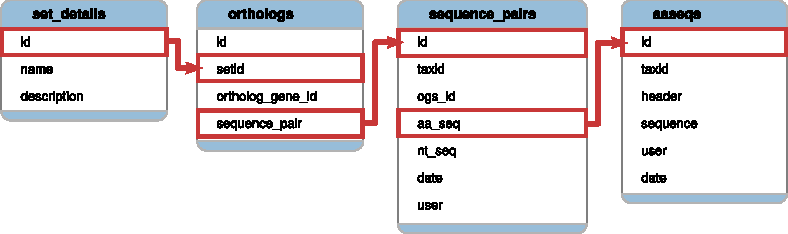
\includegraphics{img/db-orthoset.pdf}
	\caption[Database table connections for a given ortholog set]{
		\pname database structure for a given ortholog set. Each rounded rectangle
		represents a table with named columns. The red path delineates the
		\code{JOIN} query structure that returns all amino acid sequences (stored in
		the table ``aaseqs'') that belong to a given ortholog set. Ortholog set
		information is stored in the table ``set\_details''.
	}
	\label{fig:db-orthoset}
\end{figure}


\begin{figure}[ht]
	\centering
	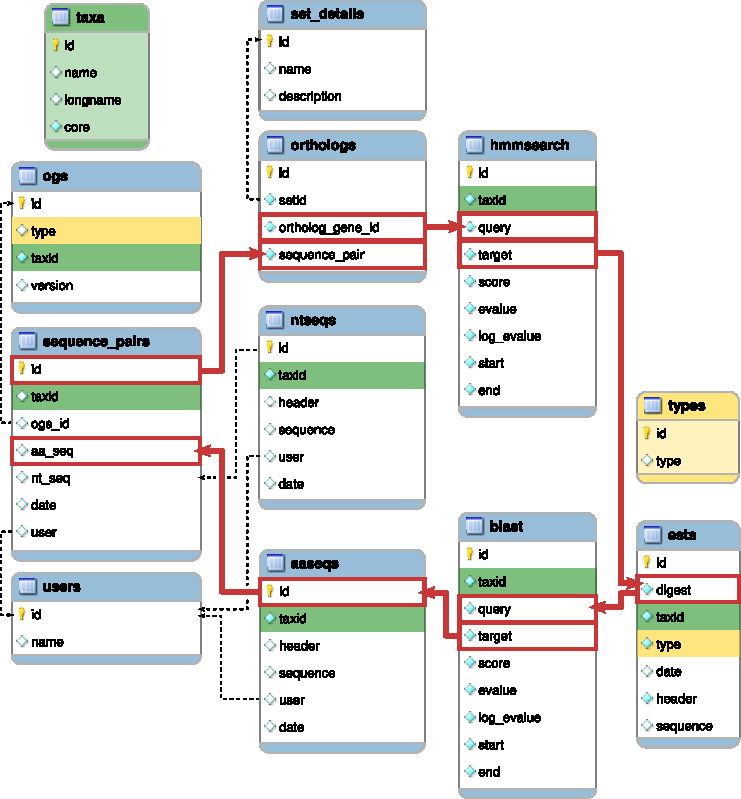
\includegraphics[width=\textwidth]{img/dbstructure.pdf}
	\caption[\pname database structure]{
		\pname database structure. Each rectangle represents a table with named
		columns. Note the circular path (red) that can be drawn across the tables and
		that is used in \code{JOIN} queries in order to construct a graph of
		orthologous relationships. Green table columns are referenced to the ``taxa''
		table, and yellow table columns are referenced to the ``types'' table. Dotted
		lines are secondary references.
	}
	\label{fig:dbstructure}
\end{figure}




	\section{Algorithm}
		\label{sec:algorithm}
The \pname package consists of three separate tools:

\begin{description}
	\item[orthograph-manager] is a helper application intended for management of
		the database. It is intended to create the initial database structure, upload
		ortholog set and nucleic or amino acid sequence data and manage present
		ortholog sets.
	\item[orthograph-analyzer] is the actual pipeline that performs the
		bidirectional searches using \tool{hmmsearch} and BLAST. It loads the
		results into the database, but does not attempt to infer ortholog
		relationships. 
	\item[orthograph-reporter] is the reporting program that fetches the data that
		orthograph-analyzer stored in the database and establishes ortholog
		relationships by means of an iterative algorithm (see
		\autoref{sec:algorithm-reporting})
\end{description}

The decision to implement three different tools  has advantages over a
monolithic design, where a single application would do every task: database
management is separated from the actual analysis. This distinction is of
particular importance when running \pname in a multi-user environment where the
researcher does not have administrative access to the computer or the database
server. Here, the system administrator can manage the database with
orthograph-manager and provide the researcher with the required environment for
analysis. No knowledge of Perl or SQL is required.

The separation of searching and reporting algorithms into discrete programs is
beneficial because it facilitates implementation of different analysis
strategies. The data in the database can be evaluated in multiple ways without
having to run the searches again. Orthograph-reporter provides the algorithm for
predicting gene orthology that is described in
\autoref{sec:algorithm-reporting}, but for a different question, the data may be
assessed under a different algorithm or with different criteria. This versatile
implementation provides programmers and researchers alike with a flexible
framework for analyses on multiple levels. 

The searching and reporting programs can be chained into a single run with a
simple batch script. The configuration file-driven design facilitates this: a
single configuration file contains the necessary information for all \pname
programs.

In the following subsections, the algorithms for analysis and evaluation are
outlined in detail.

		\subsection{Analysis}
			The analysis algorithm is as follows:

\begin{enumerate}
	\item Get configuration, initialize global variables.
	\item Check the following:
	\begin{enumerate}
		\item Do the user settings make sense? If not, exit.
		\item Are the paths to the input file and the programs correct? If not,
			exit.
		\item Do the output directories exist? If not, create them.
		\item Does the database structure exist? If not, exit.
	\end{enumerate}
	\item Backup old results, if requested.
	\item Clear old results from file system and database, if requested.
	\item Create the HMMs, if they do not exist.
	\item Create the BLAST database of all core taxa, if it does not exist.
	\item Translate the input file in all six reading frames, if it is nucleic
		acid data.
	\item Load the translated sequences into the database, generating unique
		SHA256 digests on the way.
	\item Get all translated sequences of the target species from the database.
		Sequence identifiers are now SHA256 digests. Write the sequences into a
		temporary file.
	\item For each HMM, do the following:
	\begin{enumerate}
		\item Search the translated sequences in the temporary file with this HMM.
			Skip to the next HMM if no hits were obtained. Otherwise, read the tabular
			search report and store it in the database. 
		\item For each hit, do the following:
		\begin{enumerate}
			\item Get the hit sequence from the database and write the relevant
				subsequence to a Fasta file. This information has been gained from the
				hmmsearch report file.
			\item Search this sequence against the BLAST database. Skip to the next
				HMM if no hits were obtained. Otherwise, read the tabular search report
				and store it in the database. 
		\end{enumerate}
	\end{enumerate}
\end{enumerate}

Note that the analysis algorithm does not imply ortholog relationships. Only the
bidirectional searches are performed during this step. 

		\subsection{Evaluation}
			\label{sec:algorithm-reporting}
The reporting algorithm is as follows:

\begin{enumerate}
	\item Get configuration, initialize global variables.
	\item Get a list of ortholog group IDs and their associated ortholog sequences
		from the database.
	\item Get all results in the form:
	\begin{lstlisting}
	hmmsearch_evalue => {
		ortholog_group_id => [
			reciprocal_hit,
			reciprocal_hit,
		],
		ortholog_gene_id => [
			reciprocal_hit,
			reciprocal_hit,
		],
		...
	}
	\end{lstlisting}
	\item Sort the e-values in ascending order.
	\item Starting with the lowest hmmsearch e-value, do the following:
	\begin{enumerate}
		\item For each ortholog group that has a hit with this e-value, do the following:
		\begin{enumerate}
			\item Check whether this ortholog group is present in the list that was
				generated in step 2. If not, skip to the next group (this ortholog group
				has already been assigned a transcript).
			\item Sort the reciprocal hits by BLAST e-value in ascending order.
			\item For each reciprocal hit, do the following:
			\begin{enumerate}
				\item If the reciprocal search hit a sequence that is in this ortholog
					group, and this transcript has not been assigned previously, then this
					is a valid match. Otherwise, skip to the next reciprocal hit unless
					the ``soft threshold'' has been reached (in that case, skip to the
					next ortholog group).
				\item Assign this transcript to this ortholog group if it does not
					overlap with an existing assignment. This transcript cannot be
					assigned again.
			\end{enumerate}
			\item If there is a gap between the transcripts (the end of one transcript
				lies more than 1 bp before the start of the next), fill the gap with
				'X' and concatenate the fragments.
		\end{enumerate}
	\end{enumerate}
\end{enumerate}


	\section{Implementation decisions}
		\subsection{Soft threshold}
			In \pname, not only the e-value threshold for both the \tool{hmmsearch} and
BLAST searches define a criterion that must be met in order for a transcript to
be considered orthologous to a given OG. Here, a so-called \emph{soft threshold}
is introduced: When traversing the graph by ascending \tool{hmmsearch} e-value
edges, it may happen that, for a given OG--transcript combination, multiple
BLAST searches that are consecutive in e-value did not hit an amino acid
sequence that was used to build the HMM for this OG. In \pname, the soft
threshold defines a number of reciprocal searches for a single OG that did not
fulfill the triangulation criterion. Above the soft threshold, the reliability
of this ortholog relationship is considered insufficient, and the given OG is
skipped (for that given \tool{hmmsearch} e-value). 


		\subsection{SHA-256 digests as sequence identifiers}
			Unique sequence IDs are necessary in order for \code{hmmsearch} not to create
confusion by treating whitespace in sequence headers as a description
separator. To avoid this, and to maintain a consistent naming scheme across
applications, \pname~uses a SHA-256 checksum to generate a unique ID for every
sequence. The checksum is generated using both the original header and the
sequence. Sequences are loaded into the database along with these checksums.
During the analysis, wherever a file is generated that includes sequence
identifiers, this checksum is used. This also eliminates the problem with
\code{fastatranslate} introducing whitespace that might confuse
\code{hmmsearch}.

It must be guaranteed that no two checksums, i.e., two sequence identifiers, are
ever the same. The SHA-256 hashing algorithm generates a checksum that is 160 bits,
or 40 hexadecimal characters in length. The probability $p$ of a hash collision
(i.e., two hashed elements returning the same checksum) in $n$ elements is

\begin{equation}
p \ge \frac{n (n-1)}{2} \times \frac{1}{2^b}
\label{eq:hashcollision}
\end{equation}

where $b$ is the number of bits generated by the hash function. There need to be
more than $1.7 \times 10^{15}$ objects for the SHA-256 hashes to exceed a collision
probability of $10^{-18}$. Since the hash space is expected to contain only a
number of objects in the range of $10^6$ to $10^{12}$, it is statistically safe
to assume that every checksum is unique. 



		\subsection{Performance considerations}
			\subsubsection{One BLAST database comprising all core taxa proteomes}
				\pname uses a single BLAST database comprising all reference taxa proteomes.
Only one BLAST search is performed for each HMM hit.

			\subsubsection{MySQL performance}
				\label{sec:mysql-performance}
As outlined in \autoref{sec:mysql}, MySQL was used for various reasons, one of
which is that a RDBMS is optimized for speed and efficiency. This is true
especially for small databases with tables that contain less than five million
records in this schema (see \autoref{sec:database-structure}). However, in its
current structure, without administrative access to MySQL server
variables---which allow more fine-tuning for performance
\citep{schwartz2012}---it does not scale well: above of 5 million records,
MyISAM performance for re-indexing the table after uploading new transcriptome
sequence data starts to drop noticeably (see \autoref{fig:transaction-time}). 
This problem can be circumvented by redesigning the database structure. A
possible solution is discussed in section \ref{sec:table-per-species}.

\begin{figure}[h]
\centering
\def\svgwidth{\textwidth}
\input{img/transaction-time.pdf_tex}
\caption{Transaction time}
\label{fig:transaction-time}
\end{figure}



	\section{Distributed analysis}
		The server-client model of MySQL enables a distributed analysis on a computer
network. This is advantageous on either a HPC cluster designed for massively
parallelized computing, where many physical computers are connected in a
low-latency network and communicate with each other, or a network of standard
desktop computers. In either environment, one computer (or more: in
high-performance database applications, so-called federated databases are
distributed across many servers) functions as a database server, and the others
connect to it over the network. 

\begin{figure}[h]
\centering
\def\svgwidth{0.7\textwidth}
\input{img/server-client.pdf_tex}
\caption[MySQL server-client model]{MySQL server-client model. Multiple
computers (clients) can connect to a single database server and run independent
analyses on the same data.}
\label{fig:server-client}
\end{figure}



\chapter{Discussion}
	The results are of theoretical and practical nature and shed light on how a
pipeline for orthology prediction using HMMs and a RDBMS should be designed,
including challenges and pitfalls. 
The results also highlight the high potential of an extensive, metadata-enriched
ortholog cluster graph for phylogenetic and other analyses. 

During the development of \pname, I was faced with obstacles of both theoretical
and practical nature. I gained insights into the delicacies of modern Perl
development and high-performance MySQL database implementations.

	\section{Algorithm}
		The algorithm in \pname has been distributed into three programs:
\tool{orthograph-manager}, \tool{orthograph-analyzer}, and
\tool{orthograph-reporter}. The decision to implement three different tools
has advantages over a monolithic design, where a single application would do
every task: database management is separated from the actual analysis. This
distinction is of particular importance when running \pname in a multi-user
environment where the researcher does not have administrative access to the
computer or the database server. Here, the system administrator can manage the
database with \tool{orthograph-manager} and provide the researcher with the
required environment for analysis. No knowledge of Perl or SQL is required.

The separation of searching and reporting algorithms into discrete programs is
beneficial because it facilitates implementation of different analysis
strategies. The data in the database can be evaluated in multiple ways without
having to run the searches again. \tool{orthograph-reporter} provides the
algorithm for predicting gene orthology that is described in
\autoref{sec:algorithm-reporting}, but for a different question, the data may be
assessed under a different algorithm or with different criteria. This versatile
implementation provides programmers and researchers alike with a flexible
framework for analyses on multiple levels. 

The searching and reporting programs can be chained into a single run with a
simple batch script. The configuration file-driven design facilitates this: a
single configuration file contains the necessary information for all \pname
programs (see \autoref{sec:example-config} in the appendix for an example
configuration file).


	\section{Implementation}
		During the development of \pname, I was faced with obstacles of both theoretical
and practical nature. I gained insights into the delicacies of modern Perl
development and high-performance, large-scale MySQL database design. 

		\subsubsection{User-friendliness}
			\pname is designed to be as user-friendly as possible. It is well-documented and
comes with a step-by-step guide for inexperienced users. The \pname
programs benefit from fine-tuning the MySQL server as described in, \eg,
\citet{schwartz2012} or \citet{schneider2005}. I was aware of the fact that most
users cannot be expected to change MySQL server settings. Thus, I have tried to
bypass these fine-tuning facilities by putting much consideration into the
database design. However, the best database structure cannot compensate, \eg, a
memory buffer pool that is too small for the given database and usage. This has
to be considered when deploying \pname in a production environment (see also
\autoref{sec:future-devel} for future improvements regarding the database
performance).

		\subsubsection{HMM-based forward search}
			When triangulating bidirectional best hits as explained in
\autoref{sec:orthology-howto}, an exhaustive assessment of gene orthology in
transcriptome data, using a search algorithm like BLAST, must try to align all
orthologous amino acid sequences against all transcriptome sequences.  

\pname uses HMMs for the forward search, \ie, for identification of ortholog
candidates in the query library of transcriptome sequences. However, in addition
to harnessing the power of the underlying mathematical models for obtaining
remotely similar amino acid sequences---which a similarity-based algorithm like
BLAST would not find (see \autoref{sec:hmms})---a HMM-based search offers an
additional performance value: it pools the substitution probability information
contained in a multiple sequence alignment in a single statistical model. By
using that for performing a search comprising homology information of $n$
sequences in that ortholog group, the number of required searches is reduced to
only $1$; this leads to a speedup of up to $n-1$ compared to an all-against-all
BLAST search.


		\subsubsection{Soft threshold}
		\subsubsection{SHA-256 digests as sequence identifiers}
			SHA-256 digests are generated using a cryptographic hashing algorithm described
by \citet{gallagher2008}. For a consistent and reproducible state of the
nucleotide or amino acid sequence data during all analysis steps, it must be
guaranteed that no two digests, \ie, two sequence identifiers, are ever
identical. The SHA-256 hashing algorithm generates a digest that is 160 bits, or
40 hexadecimal characters in length. The probability $p$ of a hash collision
(\ie, two hashed elements returning the same digest) in $n$ elements is

\begin{equation}
p \ge \frac{n (n-1)}{2} \times \frac{1}{2^b}
\label{eq:hashcollision}
\end{equation}

where $b$ is the number of bits generated by the hash function. There need to be
more than $1.7 \times 10^{15}$ objects for the SHA-256 hashes to exceed a collision
probability of $10^{-18}$. Since the hash space is expected to contain a number
of objects in the range of $10^6$ to $10^{12}$, it is statistically safe to
assume that every digest is unique. 


		\subsubsection{Traversing the graph by e-value}
			The \pname algorithm is different from the one that is implemented in \hamstr:
It does not assign transcript sequences to ortholog groups (OG) based on a
per-OG basis, but instead first collects all possible graph edges  and traverses
them by ascending \tool{hmmsearch} e-value (see \autoref{fig:orthograph-graph}).
This has two advantages: firstly, it assures that the transcript sequences are
mapped to the most relevant OG, and not the one that was processed first.
Secondly, by removing the transcript sequences from the list of candidate
transcripts, redundant assignment is precluded, \ie, the same transcript cannot
be mapped to multiple OGs or vice versa.

		\subsubsection{One BLAST database comprising all reference proteomes}
			In \hamstr, one BLAST database has to be maintained for each reference taxon.
This leads to the problem of BLAST scores and e-values not being normalized:
since the BLAST databases for the reference proteomes that are used in \hamstr
are of differing sizes, the e-values, which depend on the database size, cannot
be compared across reference taxa. To generate a ``normalized'' score and
e-value, \hamstr takes an additional comparison step using a pairwise alignment
with ClustalW.

In contrast to \hamstr, \pname uses one BLAST database comprising all reference
taxa proteomes. E-values are comparable across taxa since the database is of
constant size. Additionally, only one BLAST search is required instead of $n$
searches, where $n$ is the number of reference taxa. This leads to a potential
performance boost of up to $n-1$ compared to \hamstr.

		\subsubsection{Distributed analysis}
			\label{sec:distributed-analysis-discussion}
When using a multi-client setup with standard desktop computers like described
in \autoref{sec:distributed-analysis}, it is beneficial to designate one
computer exclusively for the MySQL server instance, and not run additional
\pname analyses on that machine. The large amount of data that is sent to and
from the server, and the overhead due to table indexing take up the majority of
the CPU capacity. In order to not hinder the other computer's analysis
performance, the server computer should be able to dedicate its entire resources
to managing the MySQL database (\ie, no \pname analysis should be running on the
server itself). The MySQL server itself is multithreaded and scales well over
multiple processors. It can handle hundreds of simultaneous connections per
second without problems. The InnoDB storage engine benefits from large amounts
of RAM because it can cache portions of a table in RAM and thus does not have to
access the hard drive frequently \citep{schneider2005}.

When planning an integration of \pname in a HPC environment, additional factors
have to be considered. HPC clusters are optimized to provide a high computing
capacity by relying on a massively parallelized architecture. MySQL database
servers, especially when running large InnoDB engine tables exclusively, benefit
the most from a large memory pool. However, memory is valuable for all
applications that run on HPC clusters, and allocating a large portion of the
available memory to the database server is not feasible. Thus, the database
server must be externalized (see \autoref{fig:cluster} for a possible
configuration). This requires a low-latency network connection so that the
database connection does not become a performance bottleneck.

\begin{figure}[h]
	\centering
	\def\svgwidth{0.8\textwidth}
	\input{img/cluster.pdf_tex}
	\caption[Possible integration of a database in a grid computing environment]{
		Possible integration of a database server in a grid computing environment. In
		a computing grid, the individual compute nodes communicate with each other
		and exchange data. They are coordinated by the control node, which is the only
		interface to both the user and the database.
	}
	\label{fig:cluster}
\end{figure}


		\subsubsection{MySQL performance}
			\label{sec:mysql-performance-discussion}
During testing, MySQL performance became a bottleneck because of the re-indexing
issues of MyISAM, which take increasingly long with growing table size
(see subsection \autoref{sec:mysql-performance}. A solution to this issue is to
partition the tables ``ests'', ``hmmsearch'', and ``blast'' into individual
tables for each query dataset. Transcriptome sequence data as generated within
the 1KITE project have a number of sequences in the order of $10^5$ to
$5\times10^5$, which amounts to the same number of records in the database. That
means, in the worst case, the database in its current form and without
administrative access to server variables can only store up to about ten query
datasets before it becomes slow.

Besides the indexing strategy and the query design, the database structure plays
a major role in terms of performance. Especially the tables ``hmmsearch'' and
``blast'' become excessively large after a few analyses: with an ortholog set of
4,000 OGs, if each of the 4,000 HMM searches obtains an average of 20 hits
during the HMM search, and each of the 20 BLAST searches obtains an average of
50 hits, this amounts to $4,000 \times 20 = 8 \times 10^4$ rows in the table
``hmmsearch'' and $4 \times 10^6$ rows in the table ``blast''.  The rows
themselves do not contain much data (only 131 B on average), but due to the
large number of records, InnoDB performance with the current schema does not
scale well. Insertion of new data does not become noticably slow; however,
deleting old analysis results takes very long. The InnoDB cluster index
physically orders the table based on the primary key or the first unique key it
can utilize. When one row is removed, the entire table is reordered on the hard
drive for speed and defragmentation. With increasing table size, this operation
takes exponentially long (\autoref{fig:delete-time}).

The simplest and most performant solution to this problem is to create
individual tables for each query taxon. Deleting and recreating a table is much
faster than deleting a large portion out of a huge table, especially when there
are indices involved. 

\begin{figure}[h]
	\centering
	\def\svgwidth{0.4\textwidth}
	\input{img/delete-time.pdf_tex}
	\caption[Deletion time on large InnoDB tables]{
		InnoDB performance on deleting rows in large tables with many indices. With
		increasing table size, the transaction takes longer because the InnoDB
		cluster index has to physically reorder the table contents on the hard
		drive.
	}
	\label{fig:delete-time}
\end{figure}


	\section{Conclusion and outlook}
		\pname---a newly developed pipeline for gene orthology prediction in
transcriptome sequence data---was developed in the framework of this diploma
thesis. It follows a graph-based approach using hidden Markov models (HMMs) that
was implemented in its archetype software \hamstr. In the present thesis, the
concept of gene orthology was outlined and different strategies of orthology
assessment were compared. The pipeline algorithm was explained as well as
technical challenges and pitfalls highlighted. Different techniques have been
employed to overcome practical and theoretical obstacles. The result is a
modern, actively developed software pipeline that combines the power of HMMs
with state-of-the-art technology.


		\subsection{Future development}
			At the time of this writing, the tables ``ests'', ``hmmsearch'' and ``blast''
are filled in a cumulative fashion, \ie, they contain data from all query
species. This affects performance because without administrative access to
server configuration and tuning variables, a too small InnoDB key buffer along
with very large tables becomes a performance bottleneck \citep{mysql2013}. For
this reason---and because \pname is intended for users with no knowledge about
MySQL administration, and therefore fine-tuning of server variables in order to
adapt to the amount of data at hand is not possible---future development will
implement separate tables for each query dataset. This ensures high database
performance. With complex SQL queries, it will still be possible to connect
multiple datasets.


			\subsubsection{Individual analysis tables per query dataset}
				\label{sec:table-per-species}
At the time of this writing, the tables ``ests'', ``hmmsearch'' and ``blast''
are filled in a cumulative fashion, \ie, they contain data from all query
species. This affects performance because without administrative access to
server configuration and tuning variables, a too small InnoDB key buffer along
with very large tables becomes a performance bottleneck \citep{mysql2013}. For
this reason---and because \pname is intended for users with no knowledge about
MySQL administration, and therefore fine-tuning of server variables in order to
adapt to the amount of data at hand is not possible---future development will
implement separate tables for each query dataset. This ensures high database
performance. With complex SQL queries, it will still be possible to connect
multiple datasets.

This practice also alleviates the pressure on the SHA-256 digests to be unique:
in a smaller object space, the probability of a hash collision decreases
significantly.

			\subsubsection{Reciprocal HMM search}
				As hinted in the introduction (\autoref{sec:improvements}), using BLAST for the
reciprocal search step may be interpreted as a waste of specificity: why put
effort into employing HMMs for their capability of finding remotely related
amino acid sequences during the forward search, when the candidate ortholog may
be discarded later because BLAST is much stricter than a HMM search? This design
decision in \hamstr is puzzling, but alternative search algorithms could not
easily be implemented in the pipeline. This has changed with \pname: its modular
design facilitates extension and also switching to a different reciprocal search
algorithm in order to test whether the employment of a HMM-based tool for both
search directions might provide better results.

	\section{Summary}

\clearpage

%
% acknowledgements
%
\phantomsection
\addcontentsline{toc}{chapter}{Acknowledgements}
\chapter*{Acknowledgements}
	%I thank Bernhard Misof for commiting this project to me, for helpful comments
and for maintaining such a great atmosphere in this working group.

Thanks to Oliver Niehuis for really good supervising and helpful discussions.
Your challenges made me outgrow my own boundaries.

I also thank Karen Meusemann for being a brilliant office-mate, for interesting
discussions, and for forming a great team. You made my diploma year.

Thanks to Alex Donath, Julia Schwarzer, Sandra Meid, Patrick Kück, Caro Greve,
Ralph Peters, Christoph Mayer, Jeanne Wilbrandt, Tanja Ziesmann, and Hannes
Jäkel for contributing to a good working group. Without all of you this year
wouldn't have been the same.

I also acknowledge Torsten Struck, who was the first to point out the redundant
assignment bug in \hamstr, and the helpful programming community at
\url{stackoverflow.com}, which helped me with tough questions concerning Perl
and MySQL, as well as Peter Grobe, whose concrete advice helped in designing the
database.

Thanks to Silvio Philipp as well as Alf and Monika Sibla for their friendship
and for taking my mind off everything else for a few hours each Wednesday. 

Many thanks to Hannah for making me smile every day, taking care of everything
and enduring my absent-mindedness the last few weeks. 

	\clearpage

%
% bibliography
%
\phantomsection
\addcontentsline{toc}{chapter}{Bibliography}
% uncomment these four lines if using bibtex
\footnotesize
\bibliographystyle{plainnat}
\bibliography{bib/diploma}
\normalsize
% uncomment this line if using biblatex
%\printbibliography
\clearpage

%
% appendix
%
\phantomsection
\appendix
\chapter{Appendix}
	\section{Listings}
		\begin{table}[h]
\caption{Programs developed in the present thesis. The complete source code can
be found on the CD that is appended to the first referee's copy. In addition,
the most current version is hosted on GitHub (\url{https://github.com/mptrsen/Orthograph}).}
\centering
\begin{tabular}{l l}
\hline
Program name        & description \\
\hline
orthograph-manager  & Manages \pname database \\
orthograph-analyzer & Searches query data and stores results in \pname database \\
orthograph-reporter & Evaluates data in the database and assesses gene orthology \\
\end{tabular}
\label{tab:orthograph-programs}
\end{table}

	\clearpage
	\section{Example \pname configuration file}
		\label{sec:example-config}
\begin{verbatim}
#--------------------------------------------------
# # Orthograph config file
#-------------------------------------------------- 
#
# Comments start with a hash sign (#) and are ignored by the
# parser.  This way you can comment out lines you don't
# need, but would like to keep in your config file because
# they might be important later.
#
# Settings in UPPER-CASE must be changed to your local
# environment. Settings in lower-case are sane defaults.

#--------------------------------------------------
# Important stuff first. These settings are mandatory.
#-------------------------------------------------- 

#
# # MySQL connection settings.
#
mysql-username     = USERNAME
mysql-password     = PASSWORD
mysql-database     = DATABASE

# The path to your transcriptome data file. It is always
# best to use absolute paths. You may only supply one file,
# not a directory of files.
estfile            = FASTAFILE

# Species name. Make sure to pick a unique name because
# otherwise results get mixed up. You can, however, supply
# an existing name if you want to add sequences to an
# existing data set. 
species-name       = TEST-SPECIES

# The ortholog set you created earlier.
ortholog-set       = SETNAME

# Reference taxa. Must be a comma-separated list of taxa
# that are present in your ortholog set. If you don't
# specify any reference taxa (i.e., comment out this
# setting), all taxa in your set are used as reference taxa. 
reference-taxa     = COMMA, SEPARATED, LIST

# This is where your results are placed. Will be created if
# it doesn't exist.
output-directory   = /PATH/TO/OUTPUT-DIR


#--------------------------------------------------
# Options. These settings are optional, but may be
# required if the #defaults don't do.
#-------------------------------------------------- 

#
# # Paths to the programs. It's best to set absolute paths.
#
# Default alignment program; used to create the ortholog
# set. Must accept a fasta input file as input and produce
# fasta-formatted output on STDOUT.  Note: The --anysymbol
# option makes MAFFT accept any character in a sequence,
# INCLUDING '*' for stop codons and 'U' for Selenocystein.
# If you are not OK with this, you may remove the
# --anysymbol option from the command, but then it is your
# responsibility to make sure that your ortholog set
# sequences do not contain any nonstandard symbols that may
# make MAFFT choke on your set.
#
# Standard amino acid symbols are: ACDEFGHIKLMNPQRSTVWY and
# X for ambiguity.
alignment-program = mafft --localpair --maxiterate 1000 --anysymbol

# HMMbuild is used to build the profile HMMs. Part of the
# HMMER3 package.
hmmbuild-program     = hmmbuild

# makeblastdb is used to build the BLAST database. Part of
# NCBI BLAST+
makeblastdb-program  = makeblastdb

# Fastatranslate is part of the Exonerate package and
# translates the transcript sequences into all six reading
# frames. You are free to use different programs, though.
translate-program    = fastatranslate

# HMMsearch, of course. Also part of the HMMER3 package.
hmmsearch-program    = hmmsearch

# BLAST. Should be blastp from the NCBI BLAST+ package.
blast-program        = blastp

# Exonerate. 
exonerate-program    = exonerate

#
# # MySQL settings
#
# The database server. Change this if the database does not
# run on the same computer as the analysis. Ask your
# administrator if you don't know what to write here.
# Defaults to 127.0.0.1.
#mysql-dbserver             = 127.0.0.1

# Prefix for your Orthograph database tables. Useful if you
# are running multiple instances of Orthograph on the same
# database but don't want the data to be mixed up. Defaults
# to 'orthograph'.
#mysql-prefix = orthograph

#
# # Settings that affect the HMM and BLAST searches.
#
# E-value threshold. The HMMsearch e-value threshold affects
# the specificity of the HMM search, the first step in the
# reciprocal algorithm. It defines how distantly related
# candidate orthologs may be when searching through the
# transcriptome file. The BLAST e-value threshold affects
# the second step, the reciprocal search. Basically, this
# defines the false-positive probability (lower e-value =
# lower probability).
hmmsearch-evalue-threshold = 1e-05
blast-evalue-threshold = 1e-05

# You can also set a score threshold. A higher score means a
# better match. For HMMsearch, E-value and score thresholds
# are mutually exclusive. If both are set, the E-value
# threshold will be used (to use the score threshold, you
# have to unset the E-value threshold). BLAST accepts both
# E-value and score thresholds simultaneously.
#hmmsearch-score-threshold = 10
#blast-score-threshold     = 10

# Maximum number of HMMsearch hits to consider. This setting
# is useful to limit the number of reciprocal searches for
# very large number of HMMsearch hits.  However, it is also
# useful to limit the scope of your HMM searches, which you
# normally don't want to do. Unless you have an idea of how
# many reciprocal searches are required to effectively
# verify or reject a candidate ortholog, don't change this
# setting.  Defaults to 1000.
#max-blast-searches         = 1000

# The soft threshold is a special concept of Orthograph:
# While checking in strict mode (see below) whether the
# reciprocal hits are part of the ortholog group in
# question, this many mismatches may occur before the
# ortholog candidate is rejected.  Defaults to 5.
#soft-threshold             = 5

# Maximum number of BLAST hits to consider for ortholog
# candidates.  Defaults to 100.
blast-max-hits             = 100

# 
# # Other options
#
# Strict search. Normally it is enough for a match to occur
# if one of the reference taxa is hit in the reciprocal
# search. In strict mode ALL reference taxa must be hit to
# verify an ortholog assignment. This is (much) more
# conservative.
#strict                      = 1

# Clear pre-existing data of the same species from the
# database prior to the analysis. Recommended if you plan to
# run the same analysis multiple times, but doesn't hurt
# otherwise.  This is the default, uncomment this line if
# you want to turn it off.
#clear-results-from-database = 0

# Delete old result files. This means the HMMsearch and
# BLAST report files found in the output directory. If you
# plan to run the same analysis multiple times with the same
# HMMsearch and BLAST settings, then don't have them
# deleted. This will speed up the process significantly,
# since the search programs don't have to be run again.
# This is the default. Uncomment this line if you want the
# files deleted.
#clear-result-files          = 1

# Selenocysteine (U) may occur in some protein sequences.
# However, some alignment programs do not accept this
# nonstandard amino acid symbol. You can tell Orthograph to
# substitute all 'U' in the sequences with a different
# character. The default is not to substitute.
#substitute-u-with           = X

# Verbose output. More information about the HMMsearch and
# BLAST hits. Normally you don't want to see this. If you
# are really interested in what Orthograph is thinking
# during the analysis, uncomment this. Verbose and quiet are
# mutually exclusive.
#verbose                     =  1

# Quiet output. Uncomment this if you don't want to be
# bothered during the analysis. Verbose and quiet are
# mutually exclusive.
#quiet                       = 1


#
# # More paths
# 
# Sets directory. Useful if you would like to keep your
# ortholog sets (that is, the BLAST database, the HMMs and
# the alignment files for each ortholog gene) in a separate
# place. Defaults to 'sets' (in the current directory).
#sets-dir    = /PATH/TO/SETS/DIR

# Log file. If set, all messages will also be written to
# this file. If this is not set, messages are not written to
# a log file, but to STDOUT and STDERR.
#logfile = /PATH/TO/LOGFILE
\end{verbatim}

	\clearpage

\end{document}
% EOF
